\documentclass[10pt]{beamer}
%\documentclass[10pt,handout]{beamer}
\usepackage[spanish]{babel}
\usepackage[utf8x]{inputenc}
\usepackage{amsmath}
\usepackage{amsfonts}

%\usetheme{Frankfurt}
%\usetheme{Ilmenau}
%\usetheme{Luebeck}
\usetheme{Madrid}
%\usetheme{Warsaw}

\title[Identificaci\'on de Letras Utilizando Bubbles]{Detecci\'on de Rasgos en la Identificaci\'on de Letras Utilizando Bubbles}
\subtitle{Intr. a Neurociencia Cognitiva y Computacional}
\author[Miguel, Mail\'en, Christian]{Christian Cossio Mercado,\\Mail\'en G\'omez Mayol,\\Miguel Mart\'inez Soler}
\institute[FCEyN,UBA]{Departamento de Computaci\'on - FCEyN, UBA}
\date{31 de mayo de 2011}


\begin{document}

\begin{frame}%<handout:0>
\titlepage
\end{frame}

\section{Introducci\'on}
  \subsection{Objetivos}
      \begin{frame}
	\frametitle{Objetivo del experimento}
	\begin{itemize}
		\item \textbf{Identificar rasgos utilizados por las personas para identificar letras presentadas en distintas tipograf\'ias}\pause
		\item \alert{¿Cómo lo hacemos?}\pause
		\begin{figure}
		  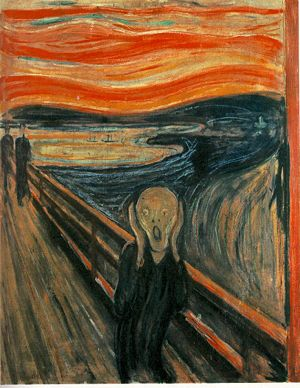
\includegraphics[height=0.5\textheight]{graficos/elGrito.jpg}
		  %\caption{Eficiencia vs complejidad para distintas tipografías}
		\end{figure}

	\end{itemize}
      \end{frame}

  \subsection{Todos Somos Sujetos}
      %estímulo máscara random
      \begin{frame}
	\frametitle{Todos Somos Sujetos}
	\begin{itemize}
		\item Vamos a intentar identificar algunas letras\ldots
	\end{itemize}

	\begin{figure}
	  
\includegraphics[height=0.7\textheight]{graficos/bubblebobble.png}
	\end{figure}
      \end{frame}

  %objetivos e hipótesis
\part[Antecedentes]{Revisi\'on de Antecedentes}
\frame{\partpage}

  \section{Antecedentes}
  %Pelli
	\begin{frame}
	\frametitle{Feature Detection and Letter Identification\\(Pelli et al., 2006)}
	\begin{columns}[t]
	\column{.60\textwidth}
	\begin{itemize}
		\item Conceptos de la identificación de letras y metodología experimental\pause
		\item Definición de complejidad (Attneave)
		  \begin{equation*}
		   \mathnormal{\text{complejidad}(l) = \frac{\text{per\'imetro}(l)^2}{\text{superficie}(l)}}
		  \end{equation*}\pause
		\item Relación eficiencia/complejidad
	\end{itemize}

	\column{.45\textwidth}

	\begin{figure}
	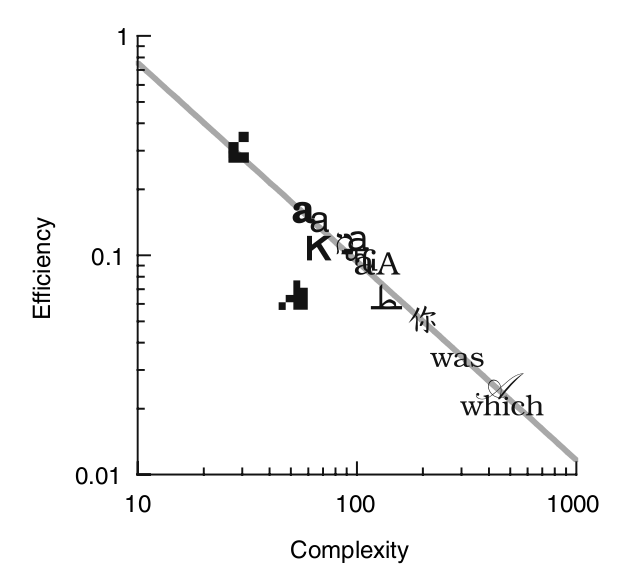
\includegraphics[width=\textwidth]{graficos/pelli4.png}
	\caption{Eficiencia vs complejidad para distintas tipografías}
	\end{figure}
	\end{columns}
  \end{frame}

%Gosselin
	\begin{frame}
	\frametitle{Bubbles: a technique to reveal the use of information in recognition task (Gosselin \& Schyns, 2001)}
	\begin{columns}[t]
	  \column{.65\textwidth}
	    \begin{itemize}
		\item Concepto de la técnica y del diseño del experimento
		\item<2->Generación de un estímulo
		    \begin{figure}
		      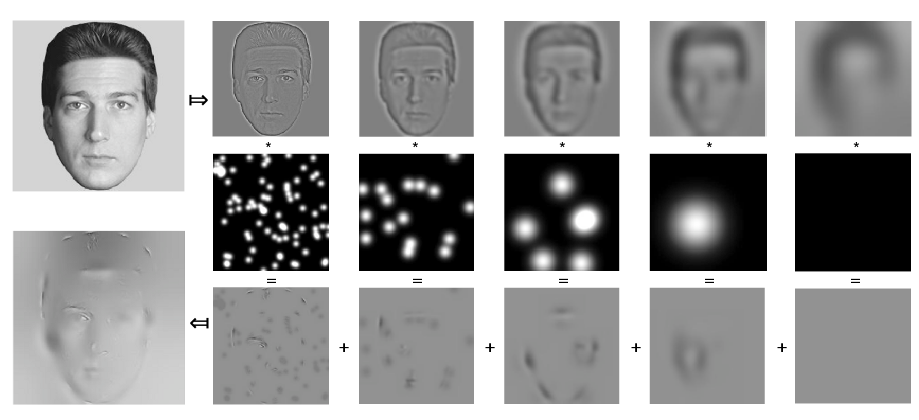
\includegraphics[width=0.9\textwidth]{graficos/estimuloGosseling.png}
		      \caption{Generaci\'on de un est\'imulo}
		    \end{figure}
	    \end{itemize}
	  \column{.35\textwidth}
	    \begin{itemize}
		  \item<2->Variables en juego
		  \only<2>{
		    \begin{itemize}
		      \item estímulo
		      \item dimensiones del estímulo
		      \item tamaño y cant. de burbujas
		      \item observadores
		    \end{itemize}
		  }
	    \end{itemize}
	    \only<3->{
		\begin{figure}
		  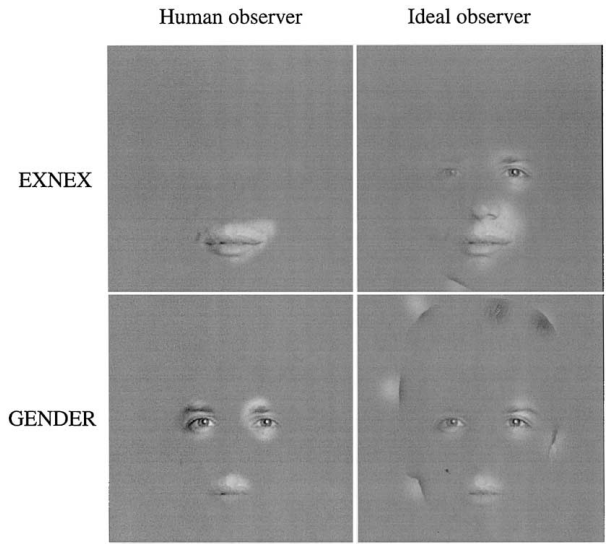
\includegraphics[width=\textwidth]{graficos/gosselin2.png}
		  \caption{Reconocimiento de expresión (ENEX) y género (GENDER)}
		\end{figure}
	    }
	  \end{columns}
	\end{frame}


	%Fiset
      \begin{frame}
	\frametitle{Features for Identification of Uppercase and Lowercase Letters (Fiset et al., 2008)}

	\begin{columns}[t]
	    \column{.4\textwidth}
	    \begin{itemize}
		\item Uso de Bubbles para identificación de letras
		\item<2-> 54 letras Arial
	    \end{itemize}	    
	  \uncover<3->{
	    \begin{figure}
		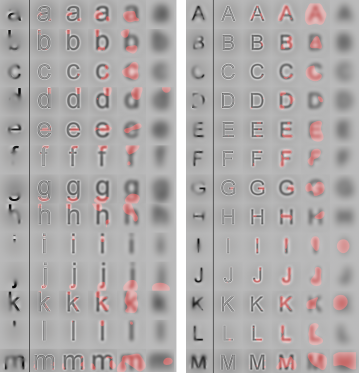
\includegraphics[width=.6\textwidth]{graficos/fiset1.png}
		\caption[Fiset et al]{Rasgos relevantes para humanos}
	    \end{figure}
	    
	    \column{.6\textwidth}
	    \begin{itemize}
		\item Humanos: Agregan 1 burbuja hasta llegar al 52\% de aciertos
		\item Obs.Ideal: Burbujas fijas, aumentan ruido hasta bajar al 52\% de aciertos
	    \end{itemize}	    
	    \begin{figure}
		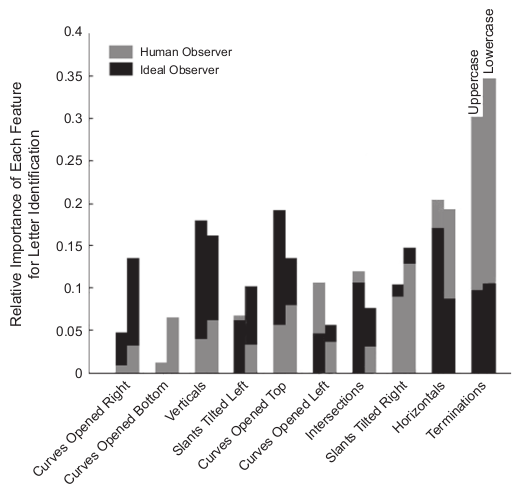
\includegraphics[width=0.5\textheight]{graficos/fiset5.png}
		\caption{Importancia relativa de los rasgos}
	    \end{figure}
	  }
	\end{columns}
      \end{frame}

\part[Experimento]{Diseño del Experimento}
\frame{\partpage}
\section{Experimento}

  \subsection{Objetivo e Hip\'otesis}
      \begin{frame}
	\frametitle{Objetivo e Hip\'otesis}
	\begin{itemize}
		\item Identificar rasgos utilizados por las personas para identificar letras presentadas en distintas tipograf\'ias
      \end{itemize}	\pause
      \begin{block}{Hip\'otesis}
	  \begin{enumerate}
		\item\alert<3>{El uso de tipograf\'ias ampliamente conocidas facilita el reconocimiento de letras, aún cuando la persona no se da cuenta de ello}
		\item\alert<3>{La performance en el reconocimiento de las letras es inversamente proporcional a su complejidad}
		\item\alert<4>{Los rasgos de cada letra var\'ian de acuerdo a la tipograf\'ia que se est\'e utilizando}
		\item\alert<4>{Habrá cambios en los rasgos de la `n' por la incorporación de la `ñ'}
		\item\alert<4>{Se obtendrá rasgos similares a los encontrados en la bibliografía}
		\item\alert<4>{Un observador ideal utilizar\'a rasgos distintos a los que utiliza una persona para identificar letras}
	  \end{enumerate}
      \end{block}

      \end{frame}
  \subsection{Dise\~no}

	%Elección tipografías
	\begin{frame}
	\frametitle{Elecci\'on de tipograf\'ias}
	    \begin{figure}
		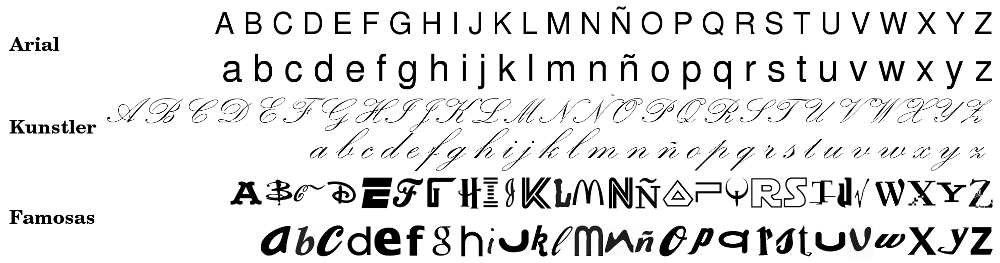
\includegraphics[width=\textwidth]{graficos/letras.png}\\ \pause
		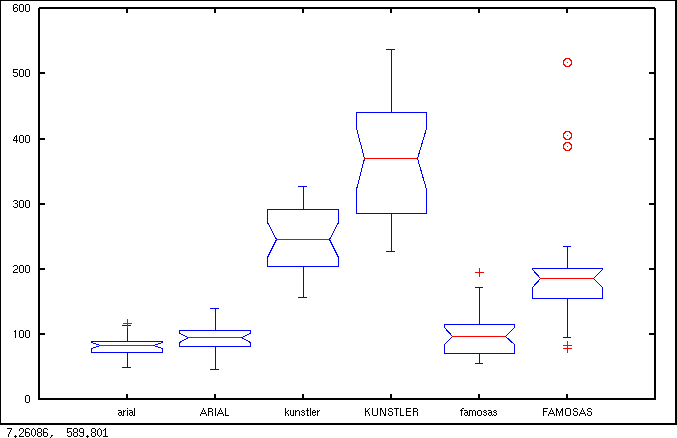
\includegraphics[width=0.8\textheight]{graficos/complejidadesBoxplot.png}
		%\caption{Tipograf\'ias y sus Complejidades}
	    \end{figure}
	\end{frame}

	%RASGOS
	\begin{frame}
	\frametitle{Definici\'on de Rasgos}
	\begin{columns} [t]
	      \column{1\textwidth}
	      \begin{figure}
		  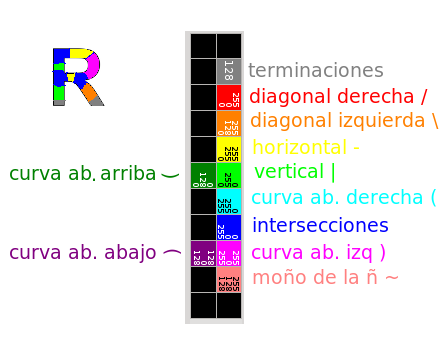
\includegraphics[height=.7\textheight]{graficos/REFERENCIA.png}
		  \caption{Identificaci\'on de rasgos para la letra \~n}
		  \end{figure}
	\end{columns}
	\end{frame}

	%estímulos
	\begin{frame}
	\frametitle{Generaci\'on de Est\'imulos}
	    \begin{figure}
	    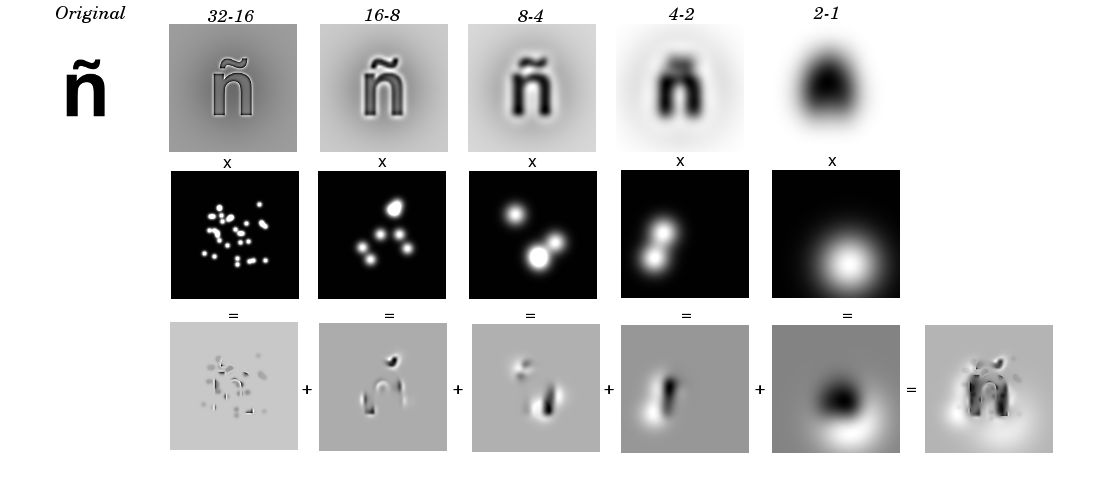
\includegraphics[width=\textwidth]{graficos/estimulofinal.png}
	    \caption{Armado del est\'imulo final}
	    \end{figure}
	\end{frame}

	%Jueves
	\begin{frame}
	\frametitle{Primer Diseño del Experimento: Jueves 12/5}
	    \begin{itemize}
		\item 13 sujetos (Gracias a todos, nuevamente!)
		\item Pocos bloques y ensayos (5 x 100, t $\approx$ 20min)
		\item Se completa una encuesta al terminar (performance, tipografías famosas)
		\item Muchas burbujas (todas las letras comienzan igual con la misma cantidad)
		\item Muy poca información {\bf:-(} (para la mayoría no se alcanza un valor cercano al 52\% de aciertos)\pause
		\item Muchos gastos en golosinas {\bf:-P}\pause
	    \end{itemize}
	\textbf{Posible Soluci\'on}: Ampliar la cantidad de ensayos y ajustar parámetros (bloques y burbujas)
	\end{frame}

	%Recauchutaje
	\begin{frame}
	\frametitle{Redise\~no del Experimento}
	    \begin{itemize}
		\item Más bloques por sujeto (17 x 100, t $\approx$ 1hr)
		\item Correcciones de errores menores (randoms, cantidad de burbujas, burbujas por banda)
		\item Mejora en la cantidad de burbujas inicial (mayor complejidad, mayor cantidad de burbujas iniciales)
		\item Filtrando casos en que no se llegó al 52\% \pause
		\item Se descartó los datos anteriores, utilizando sólo los nuevos
		\item Medimos la performance a través de tres variables
		\begin{itemize}
			\item Cant. de Burbujas ($\downarrow$)
			\item Tiempo de Respuesta ($\downarrow$)
			\item \% de Aciertos ($\uparrow$)
		\end{itemize}
    
	    \end{itemize}
	\end{frame}

	%Final
	\begin{frame}
	\frametitle{Datos Finales}
	    \begin{itemize}
		\item 6 sujetos
		\item Edades entre 21-33 años
		\item Con estudios universitarios
		\item 1700 ensayos por persona\pause
		\item Para completar datos \ldots\pause también fuimos sujetos! (2500 ensayos)
	    \end{itemize}
	\end{frame}


% El uso de tipografías ampliamente conocidas facilita el reconocimiento de letras, aún cuando la persona no se da cuenta de ello
% La performance en el reconocimiento de las letras es inversamente proporcional a su complejidad
% Los rasgos de cada letra varían de acuerdo a la tipografía que se esté utilizando
% Habrá cambios en los rasgos de la `n' por la incorporación de la `ñ'
% Se obtendrá rasgos similares a los encontrados en la bibliografía
% Un observador ideal utilizará rasgos distintos a los que utiliza una persona para identificar letras

\part{Resultados}
  \frame{\partpage}
  \section{Gr\'aficos y Tablas}
 	\begin{frame}
	\frametitle{Burbujas vs. Aciertos}
	    \begin{figure}
		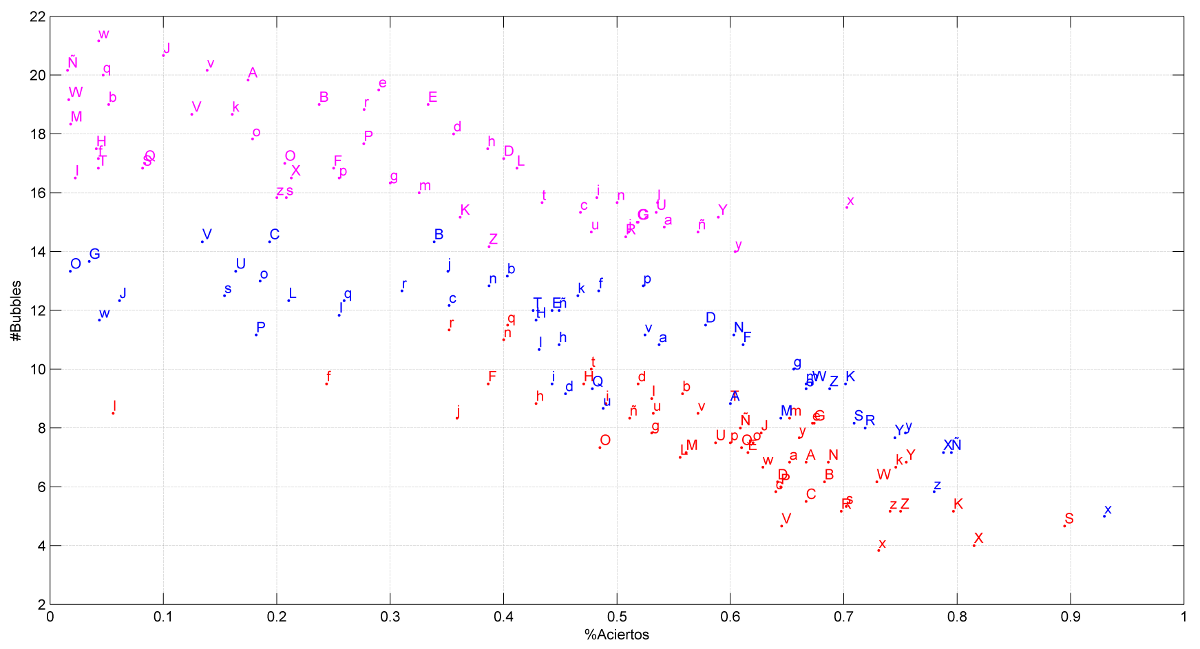
\includegraphics[width=\textwidth]{graficos/bubblesVsAciertos_Fiables.png}
		%\caption{Distribución de Tiempos de Respuesta}
	    \end{figure}
	\end{frame}

 	\begin{frame}
	\frametitle{Burbujas vs. Complejidad}
	    \begin{figure}
		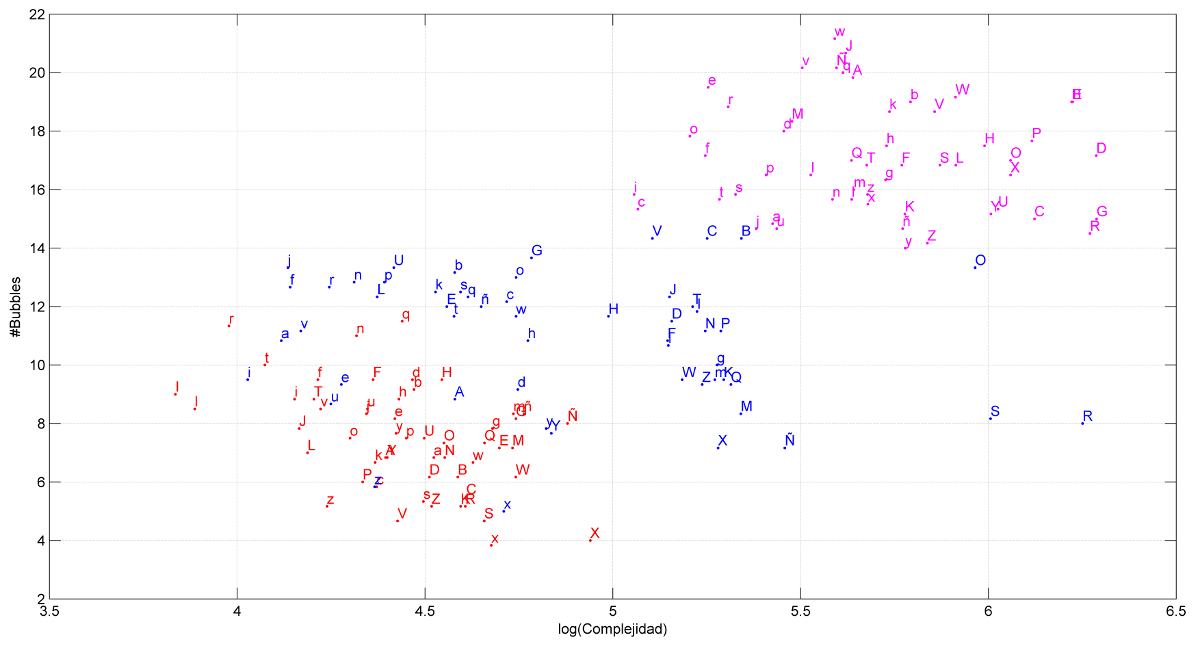
\includegraphics[width=\textwidth]{graficos/bubblesVsLogComplejidad_Fiables.png}
		%\caption{Cantidad de Burbujas vs. Log(Complejidad)}
	    \end{figure}
	\end{frame}

 	\begin{frame}
	\frametitle{Performance por Burbujas, Tipografías Famosas}
	    \begin{figure}
		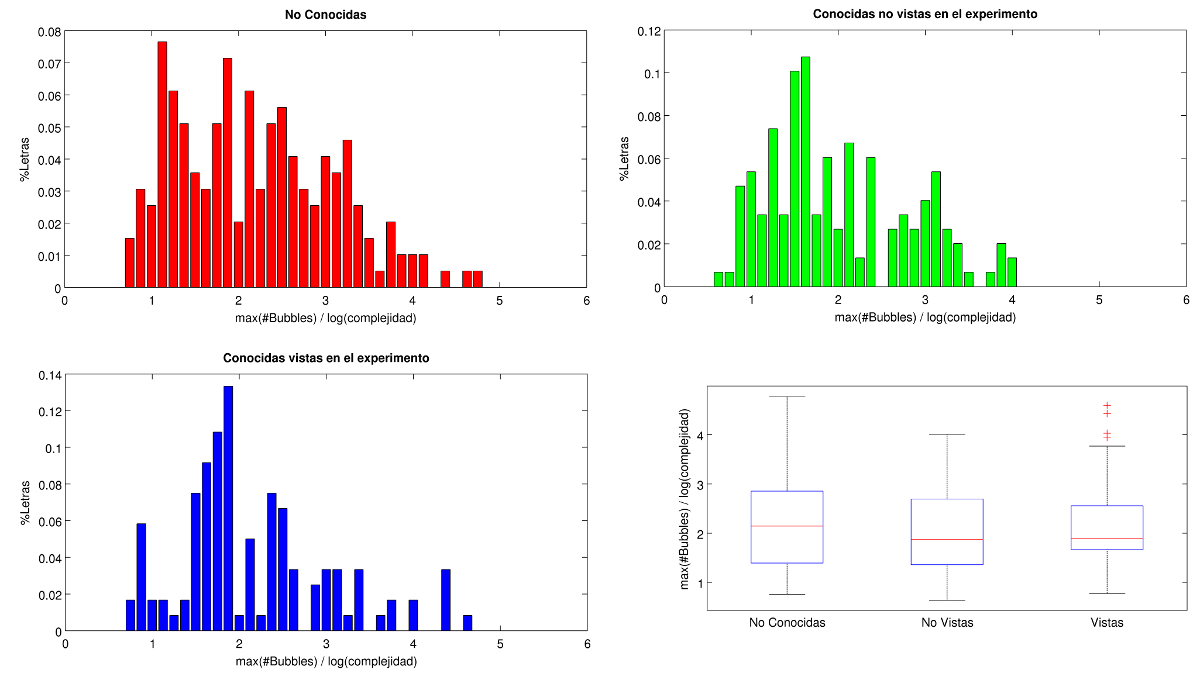
\includegraphics[width=\textwidth]{graficos/BubblesLogComplejidad_PorFamosas.png}
		%\caption{Distribución de Tiempos de Respuesta}
	    \end{figure}
	\end{frame}

   	\begin{frame}
	\frametitle{Tiempos de Respuesta}
	    \begin{figure}
		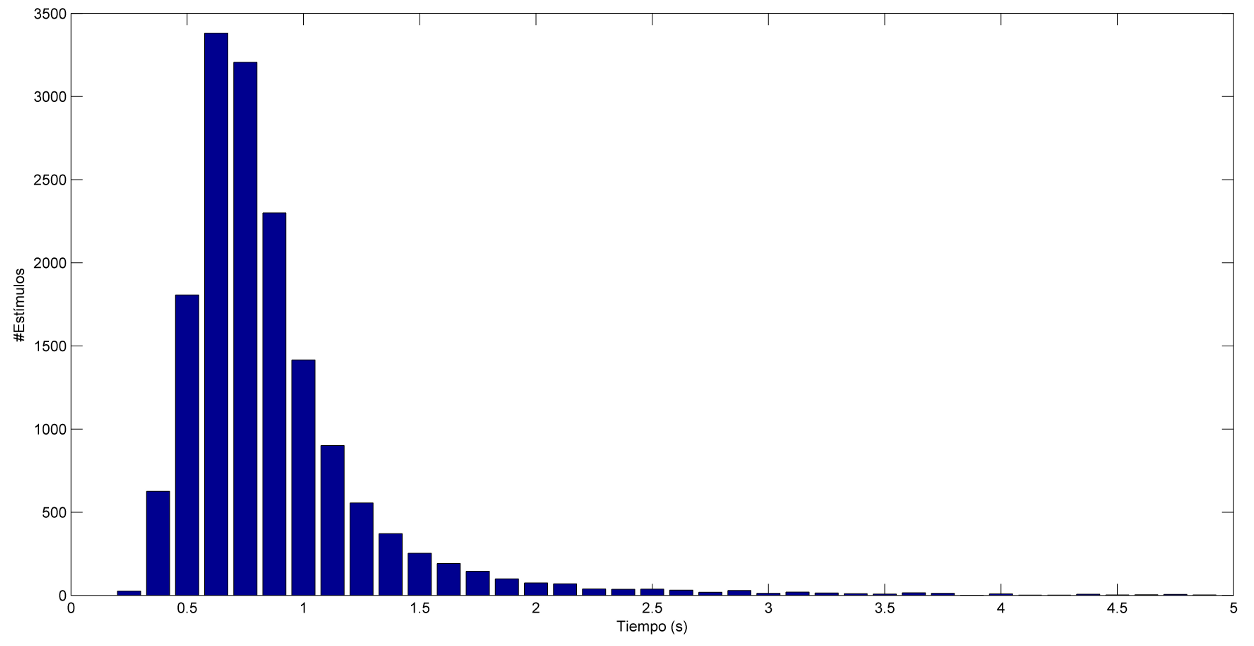
\includegraphics[width=\textwidth]{graficos/tiempoRespuesta_dist.png}
		\caption{Distribución de Tiempos de Respuesta}
	    \end{figure}
	\end{frame}

   	\begin{frame}
	\frametitle{Performance por Tiempo de Respuesta, Tipografías Famosas}
	    \begin{figure}
		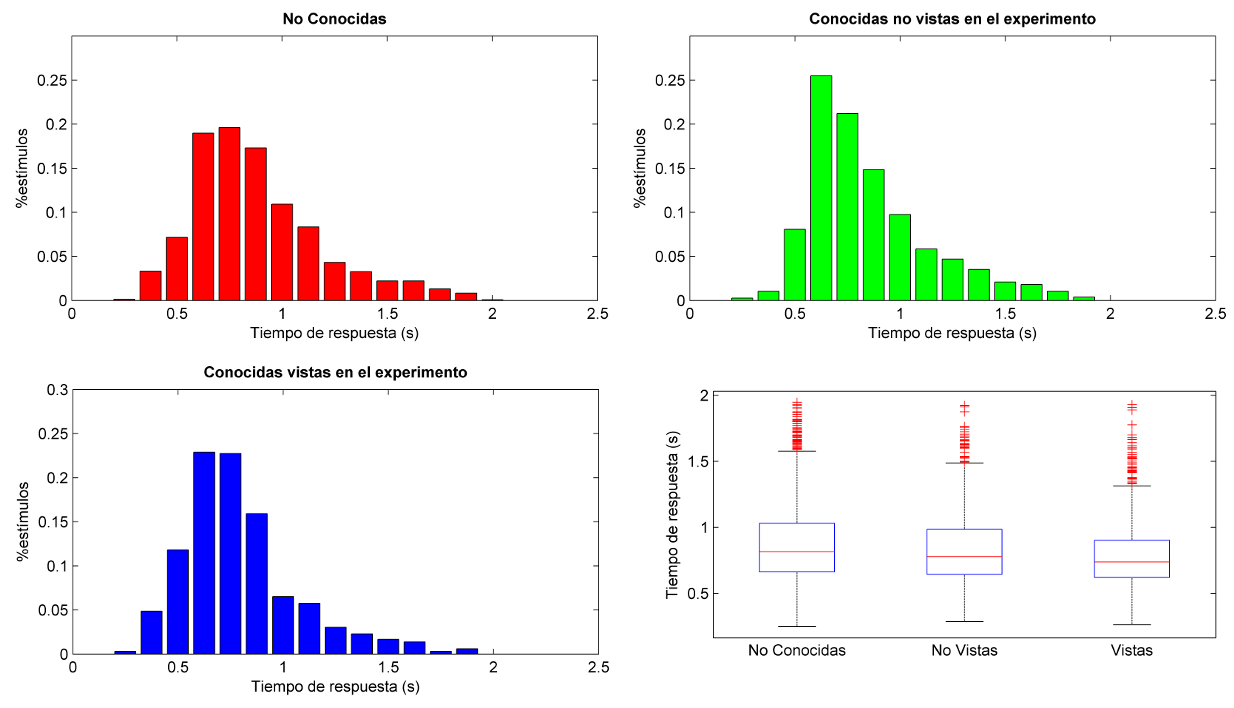
\includegraphics[width=\textwidth]{graficos/tiempoRespuesta_PorFamosas.png}
		%\caption{Distribución de Tiempos de Respuesta}
	    \end{figure}
	\end{frame}

 	\begin{frame}
	\frametitle{Rasgos Detectados}
	\begin{columns}[t]
	\column{.40\textwidth}
	\begin{figure}
	    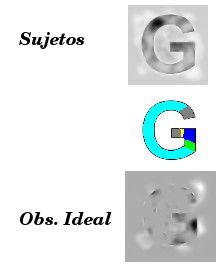
\includegraphics[width=\textwidth]{graficos/rasgos_resultadosG.png}
	    %\caption{Distribución de Tiempos de Respuesta}
	\end{figure}

	\column{.60\textwidth}
	\begin{table}
	\small
	  \begin{tabular}[t]{|r|r|r|r|r|}
		\hline
		\textbf{Id}  & \textbf{Rasgo} & \textbf{Inclusi\'on} & \textbf{Imp.Relativa} \\ \hline
		r1 & Terminaciones	& 0.76 &  0.140 \\ \hline
		r4 & Horizontal 	& 1.00 &  0.021 \\ \hline
		r5 & Vertical 		& 1.00 &  0.079 \\ \hline
		r6 & Cur.Ab.Der 	& 0.63 &  0.630 \\ \hline
		r7 & Intersecciones 	& 1.00 &  0.130 \\ \hline
	  \end{tabular}
	  %\caption{Rasgos para Sujetos}
	\end{table}
	\begin{table}
	\small	
	  \begin{tabular}[t]{|r|r|r|r|r|}
		\hline
		\textbf{Id}  & \textbf{Rasgo} & \textbf{Inclusi\'on} & \textbf{Imp.Relativa} \\ \hline
		r1  & Terminaciones	& 0.72 & 0.159\\ \hline
		r4  & Horizontal 	& 1.00 & 0.025\\ \hline
		r5  & Vertical 		& 1.00 & 0.094\\ \hline
		r6  & Cur.Ab.Der  	& 0.50 & 0.597\\ \hline
		r7  &  Intersecciones 	& 0.80 & 0.125\\ \hline
	  \end{tabular}
	  %\caption{Rasgos para Observador Ideal}
	\end{table}
      \end{columns}
\end{frame}

 	\begin{frame}
	\frametitle{Rasgos para `n' vs. `\~n'}
	  \begin{columns}[t]
	  \column{.40\textwidth}
	  \begin{figure}
	      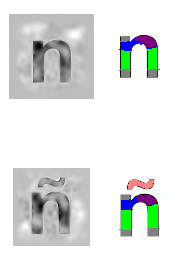
\includegraphics[width=\textwidth]{graficos/rasgos_resultadosEnieHumano.png}
	      %\caption{Distribución de Tiempos de Respuesta}
	  \end{figure}

	  \column{.60\textwidth}
	  \begin{table}
	  \small
	    \begin{tabular}[t]{|r|r|r|r|r|}
		  \hline
		  \textbf{Id}  & \textbf{Rasgo} & \textbf{Inclusi\'on} & \textbf{Imp.Relativa} \\ \hline
		    r1  & Terminaciones	& 0.89706 & 0.23431\\ \hline
		    r5  & Vertical 	& 0.89859 & 0.40845\\ \hline
		    r7  & Intersecciones & 0.93421 & 0.18182\\ \hline
		    r11 & Cur.Ab.Abajo  & 0.85625 & 0.17542\\ \hline
	    \end{tabular}
	    %\caption{Rasgos para Sujetos}
	  \end{table}
	  \begin{table}
	  \small	
	    \begin{tabular}[t]{|r|r|r|r|r|}
		  \hline
		  \textbf{Id}  & \textbf{Rasgo} & \textbf{Inclusi\'on} & \textbf{Imp.Relativa} \\ \hline
		    r1  & Terminaciones	& 0.81771 & 0.19146\\ \hline
		    r5  & Vertical 		& 0.59674 & 0.31220\\ \hline
		    r7  & Intersecciones 	& 0.97468 & 0.18780\\ \hline
		    r9  & Moño 	 	& 0.96226 & 0.18659\\ \hline
		    r11  & Cur.Ab.Abajo  	& 0.68966 & 0.12195\\ \hline
	    \end{tabular}
	    %\caption{Rasgos para Observador Ideal}
	  \end{table}
	\end{columns}

	\end{frame}

 	\begin{frame}
	\frametitle{Identificaci\'on Humana vs. Observador Ideal}
	
	  \alert{GRAFICO DE IMPORTANCIA RELATIVA DE RASGOS POR TIPOGRAFÍA-MAY/MIN}


	\end{frame}


  \section{Conclusiones}
	\begin{frame}
	\frametitle{Conclusiones}
	    \begin{itemize}
		\item Diferencia significativa en tiempo de respuesta de letras no conocidas, conocidas y conocidas vistas
		\item Mejora en los tiempos inclusive para letras conocidas pero \emph{no vistas} vs. las no conocidas \alert{(!)}
		\item Diferencia significativa de burbujas requeridas para letra no conocidas y conocidas.
		\begin{itemize}
		    \item No se pudo demostrar la significatividad entre no conocidas y conocidas vistas en el experimento\ldots
		\end{itemize}
		\item Correlación entre log(Complejidad) y Cant. Burbujas (\alert{\bf$\uparrow$}Complejidad, \alert{\bf$\uparrow$}Cant. de Burbujas)
		\item Correlación inversa entre Cant. de Burbujas y \% de Aciertos (\alert{\bf$\downarrow$}Cant. de Burbujas, \alert{\bf$\uparrow$}\% de Aciertos)
		\item Bubbles fue una técnica interesante para recorrer espacio de búsquedas de imágenes y obtener rasgos de identificación
	    \end{itemize}
	\end{frame}

  \section{Lecciones Aprendidas}
	\begin{frame}
	\frametitle{Lecciones Aprendidas}
	    \begin{itemize}
	    \item Cantidad de ensayos por persona necesarias debe ser grande ($162000 \approx 4$ días de experimentación continua\alert{!})
	    \item Los descansos entre bloques fueron útiles para reducir el cansancio y el aburrimiento
	    \item Guardar mejor los datos obtenidos, para acelerar el procesamiento (500MB/sujeto)
	    \end{itemize}
	\end{frame}

  \section{Pendientes y Trabajos Futuros}
	\begin{frame}
	\frametitle{¿C\'omo Seguimos?}
	  \begin{block}{Temas Pendientes}
	    \begin{itemize}
		\item Aumentar la cantidad de ensayos por persona, y dividirlo en sesiones
		\item Cantidad de burbujas inicial en función de complejidad de cada letra
		\item Ajuste de cantidad de burbujas ascendente y descendente
		\item Preguntar por letras conocidas mostrando ejemplos para cada una de ellas. 
	    \end{itemize}
	  \end{block} \pause

	  \begin{block}{Trabajo Futuro}
	   \begin{itemize}
		\item Incorporación del tiempo como una dimensi\'on más (an\'alisis espacio-temporal)
		\item Bubbles para habla
		    \begin{itemize}
		      \item rasgos relevantes para el reconocimiento de hablantes
		      \item detección de rasgos para expresividad o emociones
		    \end{itemize}
	    \end{itemize}                     
	  \end{block}	    
	\end{frame}

\author[Christian, Miguel, Mail\'en]{Mail\'en G\'omez Mayol,\\Miguel Mart\'inez Soler,\\Christian Cossio Mercado}

\frame{\titlepage}

\appendix
\section{\appendixname}
    \subsection{Gr\'aficos s\'olo con Datos de Sujetos}
 	\begin{frame}
	\frametitle{Burbujas vs. Complejidad}
	    \begin{figure}
		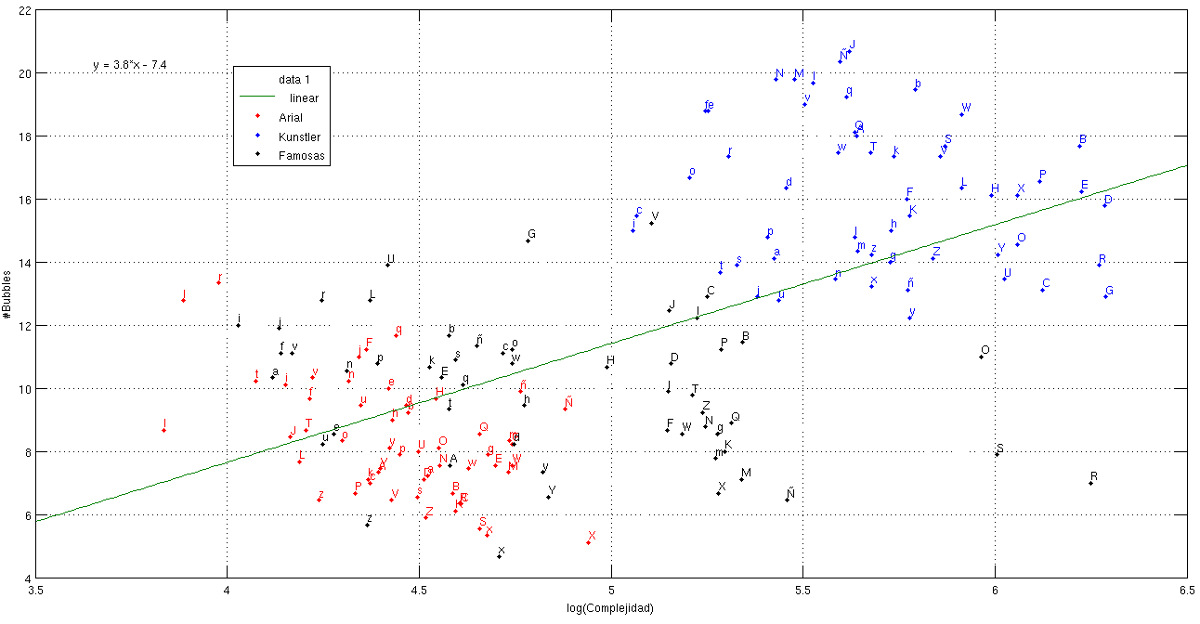
\includegraphics[width=\textwidth]{graficos/bubblesVsLogComplejidad_Todos.png}
		%\caption{Cantidad de Burbujas vs. Log(Complejidad)}
	    \end{figure}
	\end{frame}

 	\begin{frame}
	\frametitle{Burbujas vs. Aciertos}
	    \begin{figure}
		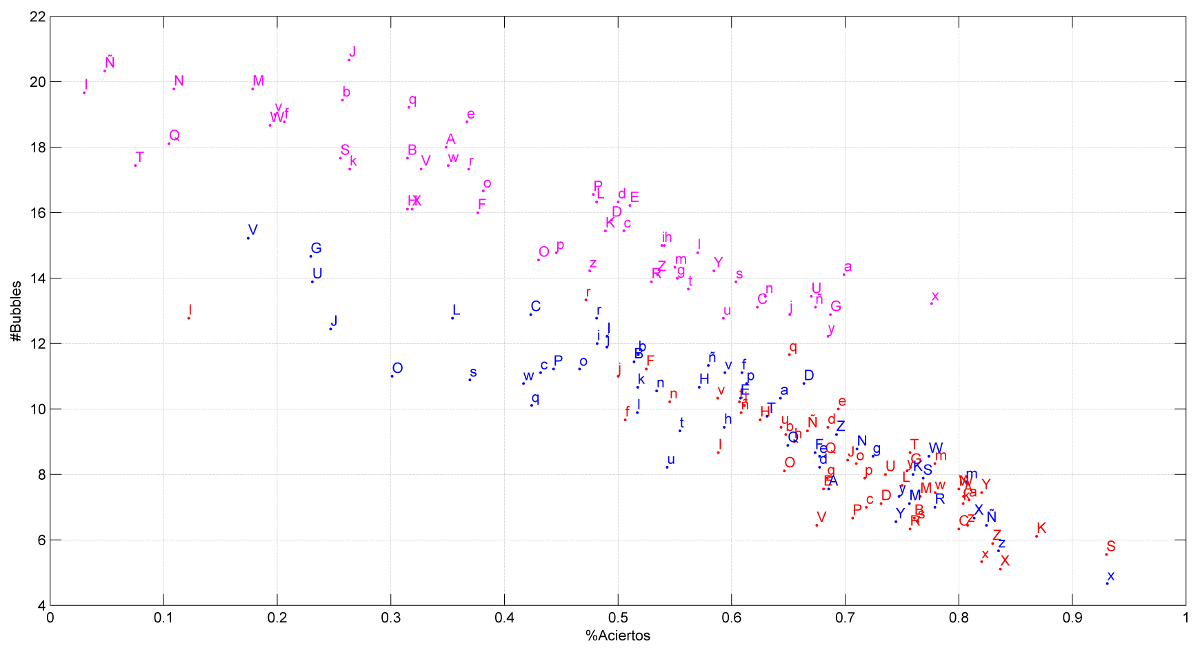
\includegraphics[width=\textwidth]{graficos/bubblesVsAciertos_Todos.png}
		%\caption{Distribución de Tiempos de Respuesta}
	    \end{figure}
	\end{frame}

    \subsection{Tests de Significatividad}

      \begin{frame}
      \tiny
	  \frametitle{Tiempo de Respuesta vs. Complejidad:\\Test de Mann-Whitney}
	\begin{table}
	  \begin{tabular}[t]{|l|l|r|r|r|}
	    \hline
		\textbf{GRUPO} & \textbf{N} & \textbf{Rango promedio} & \textbf{Suma de rangos} \\ \hline
		No Conocidas & 1439 & 1128.38 & 1623740 \\ \hline
		Conocidas & 769 & 1059.81 & 814996 \\ \hline
		\textit{Total} & 2208 &   &   \\ \hline
	  \end{tabular}   \begin{tabular}[t]{|l|r|}
	    \hline
		& \textbf{T\_RESP} \\ \hline
	      U de Mann-Whitney & 518931 \\ \hline
	      W de Wilcoxon & 814996 \\ \hline
	      Z & -2.408 \\ \hline
	      Sig. asintót. (bilateral) & 0.02 \\ \hline
	  \end{tabular}
	\end{table}

	\begin{table}
	  \begin{tabular}[t]{|l|r|r|r|}
	    \hline
		\textbf{GRUPO} & \textbf{N} & \textbf{Rango promedio} & \textbf{Suma de rangos} \\ \hline
		Conocidas & 769 & 750.4 & 577060.5 \\ \hline
		Conocidas Vistas & 660 & 673.75 & 444674.5 \\ \hline
		\textit{Total} & 1429 &   &   \\ \hline
	  \end{tabular}   \begin{tabular}[t]{|l|r|}
	    \hline
		& \textbf{T\_RESP} \\ \hline
	      U de Mann-Whitney & 226544.5 \\ \hline
	      W de Wilcoxon & 444674.5 \\ \hline
	      Z & -3.501 \\ \hline
	      Sig. asintót. (bilateral) & 0 \\ \hline
	  \end{tabular}
	\end{table}

	\begin{table}
	  \begin{tabular}[t]{|l|l|r|r|r|}
	    \hline
		\textbf{GRUPO} & \textbf{N} & \textbf{Rango promedio} & \textbf{Suma de rangos} \\ \hline
		No Conocidas & 1439 & 1104.78 & 1589772 \\ \hline
		Conocidas Vistas & 660 & 930.57 & 614178 \\ \hline
		\textit{Total} & 2099 &   &   \\ \hline
	  \end{tabular}   \begin{tabular}[t]{|l|r|}
	    \hline
		& \textbf{T\_RESP} \\ \hline
	      U de Mann-Whitney & 396048 \\ \hline
	      W de Wilcoxon & 614178 \\ \hline
	      Z & -6.114 \\ \hline
	      Sig. asintót. (bilateral) & 0 \\ \hline
	  \end{tabular}
	\end{table}
      \end{frame}

      \begin{frame}
      \tiny
	  \frametitle{Tiempo de Respuesta vs. Complejidad:\\Test de Student}
	\begin{table}
	  \begin{tabular}[t]{|r|r|r|r|r|}
	    \hline
		GRUPO & N & Media & Desviación típ. & Error típ. de la media \\ \hline
		No Conocida & 1439 & 0.8764 & 0.3082 & 0.0081 \\ \hline
		Conocida & 769 & 0.8495 & 0.2874 & 0.0104 \\ \hline
	  \end{tabular}
	  \begin{tabular}[t]{|l|r|r|r|r|r|r|r|r|r|}
	    \hline
		  & \multicolumn{2}{|c|}{Prueba de Levene} &  \multicolumn{7}{|c|}{Prueba T para la igualdad de medias} \\ \hline
		  & F & Sig. & t & gl & Sig. (bil.) & Dif. de medias & Error típ. de la dif. & \multicolumn{2}{|c|}{95\% conf. para la dif.} \\ \hline
		  &   &   &   &   &   &   &   & Inferior & Superior \\ \hline
		Varianzas iguales & 2.797 & 0.095 & 1.998 & 2206 & 0.046 & 0.0269 & 0.0134 & 0.0005 & 0.0532 \\ \hline
		Varianzas no iguales &   &   & 2.041 & 1665.884 & 0.041 & 0.0269 & 0.0132 & 0.001 & 0.0527 \\ \hline
	  \end{tabular}
	\end{table}

	\begin{table}
	  \begin{tabular}[t]{|r|r|r|r|r|}
	    \hline
		GRUPO & N & Media & Desviación típ. & Error típ. de la media \\ \hline
		Conocida  & 769 & 0.8495 & 0.2874 & 0.0104 \\ \hline
		Conocida Vista & 660 & 0.796 & 0.2779 & 0.0108 \\ \hline
	  \end{tabular}
	  \begin{tabular}[t]{|l|r|r|r|r|r|r|r|r|r|}
	    \hline
		  & \multicolumn{2}{|c|}{Prueba de Levene} &  \multicolumn{7}{|c|}{Prueba T para la igualdad de medias} \\ \hline
		  & F & Sig. & t & gl & Sig. (bil.) & Dif. de medias & Error típ. de la dif. & \multicolumn{2}{|c|}{95\% conf. para la dif.} \\ \hline
		  &   &   &   &   &   &   &   & Inferior & Superior \\ \hline
	    Varianzas iguales & 2.858 & 0.091 & 3.558 & 1427 & 0 & 0.0534 & 0.015 & 0.024 & 0.0829 \\ \hline
	    Varianzas no iguales &   &   & 3.567 & 1406.885 & 0 & 0.0534 & 0.015 & 0.0241 & 0.0828 \\ \hline
	  \end{tabular}
	\end{table}

	\begin{table}
	  \begin{tabular}[t]{|r|r|r|r|r|}
	    \hline
		GRUPO & N & Media & Desviación típ. & Error típ. de la media \\ \hline
		No Conocida & 1439 & 0.8764 & 0.3082 & 0.0081 \\ \hline
		Conocida Vista & 660 & 0.796 & 0.2779 & 0.0108 \\ \hline

	  \end{tabular}
	  \begin{tabular}[t]{|l|r|r|r|r|r|r|r|r|r|}
	    \hline
		  & \multicolumn{2}{|c|}{Prueba de Levene} &  \multicolumn{7}{|c|}{Prueba T para la igualdad de medias} \\ \hline
		  & F & Sig. & t & gl & Sig. (bil.) & Dif. de medias & Error típ. de la dif. & \multicolumn{2}{|c|}{95\% conf. para la dif.} \\ \hline
		  &   &   &   &   &   &   &   & Inferior & Superior \\ \hline
	Varianzas iguales & 11.449 & 0.001 & 5.714 & 2097 & 0 & 0.0803 & 0.0141 & 0.0527 & 0.1079 \\ \hline
	Varianzas no iguales &   &   & 5.937 & 1406.88 & 0 & 0.0803 & 0.0135 & 0.0538 & 0.1068 \\ \hline
	  \end{tabular}
	\end{table}
      \end{frame}

\end{document}